% !TEX root = ../tex/PartB.tex
\begin{frame}{PartB}
    \begin{block}{拡散モデルの基本理解}
        \begin{itemize}
            \item ノイズ付加規則を定める\\
            ノイズのないデータ→任意のノイズレベルの観測データ\\
            このように変換できる既知の規則を決める
            \vspace{1em}
            \item ノイズの付加量を学習する\\
            ノイズを含むデータからノイズのないデータの信号を推定する
        \end{itemize}
    \end{block}
    様々なノイズレベルに対してこの規則を学習すると生成にも利用可能\\
    \vspace{1em}
    生成時はノイズレベルを高い状態から低い状態へ移しながらネットワークを繰り返す\\
    ⇒データ分布の構造を徐々に備えたデータを生成できる
\end{frame}
%========================================
\begin{frame}{ノイズを含むデータの作成}
    \begin{block}{ノイズを含むバージョン}
        対象とするノイズのないデータサンプルを取り出す。
        \[
            \boldsymbol{x}_{0}\sim p_{\mathrm{data}}
        \]
        これに独立なガウスノイズを混ぜ、ノイズレベル\(t\)のデータを作る。
        \[
            \boldsymbol{x}_{t}=\alpha_{t}\boldsymbol{x}_{0}+\sigma_{t}\epsilon,
            \qquad
            \epsilon\sim\mathcal{N}(0,\mathbf{I})\footnote{$\mathbf{I}$は単位行列で、$\epsilon$は多変量正規分布に従うノイズベクトル}
        \]
        \vspace{0.1em}
    \end{block}
    \(\alpha_{t}\)と\(\sigma_{t}\)は、あらかじめ定めておく二つの係数である。\\
    $\alpha_{t}$と$\sigma_{t}$には制限をつける場合もある(e.x.分散一定の例：$\alpha_{t}^2 + \sigma_{t}^2 = 1$)\\
    ノイズレベル\(t\)において、元の信号とノイズをそれぞれどの程度混ぜるかを決める。
\end{frame}
%========================================
\begin{frame}{最も単純な選び方}
    \begin{block}{\(\alpha_{t}=1\)、\(\sigma_{t}=t\)}
        このとき、
        \[
            \boldsymbol{x}_{t}=\boldsymbol{x}_{0}+t\epsilon
        \]
        となり、\(t\)がそのままノイズの強さを表す。
    \end{block}
    \vspace{0.6em}
    \begin{itemize}
        \item \(t\)をゼロに近づけると、\(\boldsymbol{x}_{t}\)は元のノイズのないサンプル\(\boldsymbol{x}_{0}\)に近づく
        \item \(t\)を大きくすると、ノイズ項\(t\epsilon\)の影響が次第に支配的になる
    \end{itemize}
\end{frame}
%========================================
\begin{frame}{図1.3：順方向拡散}
    \centering
    \includegraphics[
        width=0.82\textwidth,
        height=0.42\textheight,
        keepaspectratio
    ]{FowardDiffusion.png}

    \vspace{0.3em}
    ノイズのないサンプル\(\boldsymbol{x}_{0}\)にノイズを加え、\\
    ノイズレベル\(t\)の観測データ\(\boldsymbol{x}_{t}\)を作る。

    \vspace{0.4em}
    \begin{exampleblock}{分布\(p_{t}\)}
        各ノイズレベル\(t\)に対して、ノイズを含むサンプルの分布\(p_{t}\)が定まる。\\
        同じ\(t\)で多数のノイズ付きサンプルを作ったとき、それらが従う分布が\(p_{t}\)である。
    \end{exampleblock}
\end{frame}
%========================================
\begin{frame}{スケジュールと分布の族}
    スケジュール\((\alpha_{t},\sigma_{t})\)は、ノイズレベルの増加に伴い、\\
    分布が元のデータ分布から単純なノイズ分布へと移るように選ぶ。
    \[
        p_{0}=p_{\mathrm{data}}
        \;\longrightarrow\;
        p_{t}
        \;\longrightarrow\;
        p_{T}\approx p_{\mathrm{prior}}
    \]
    \(p_{\mathrm{prior}}\)は通常、サンプリングが容易なガウス分布である。
    \vspace{0.6em}
    \begin{block}{分布の族}
        \[
            \{p_{t}\}_{t\in[0,T]}
        \]
        は、ノイズレベルの増加に伴って、分布が徐々に変化する様子を表す。
    \end{block}
\end{frame}
%========================================
\begin{frame}{実験：\(\alpha=1\)、\(\sigma=t\)}
    \centering
    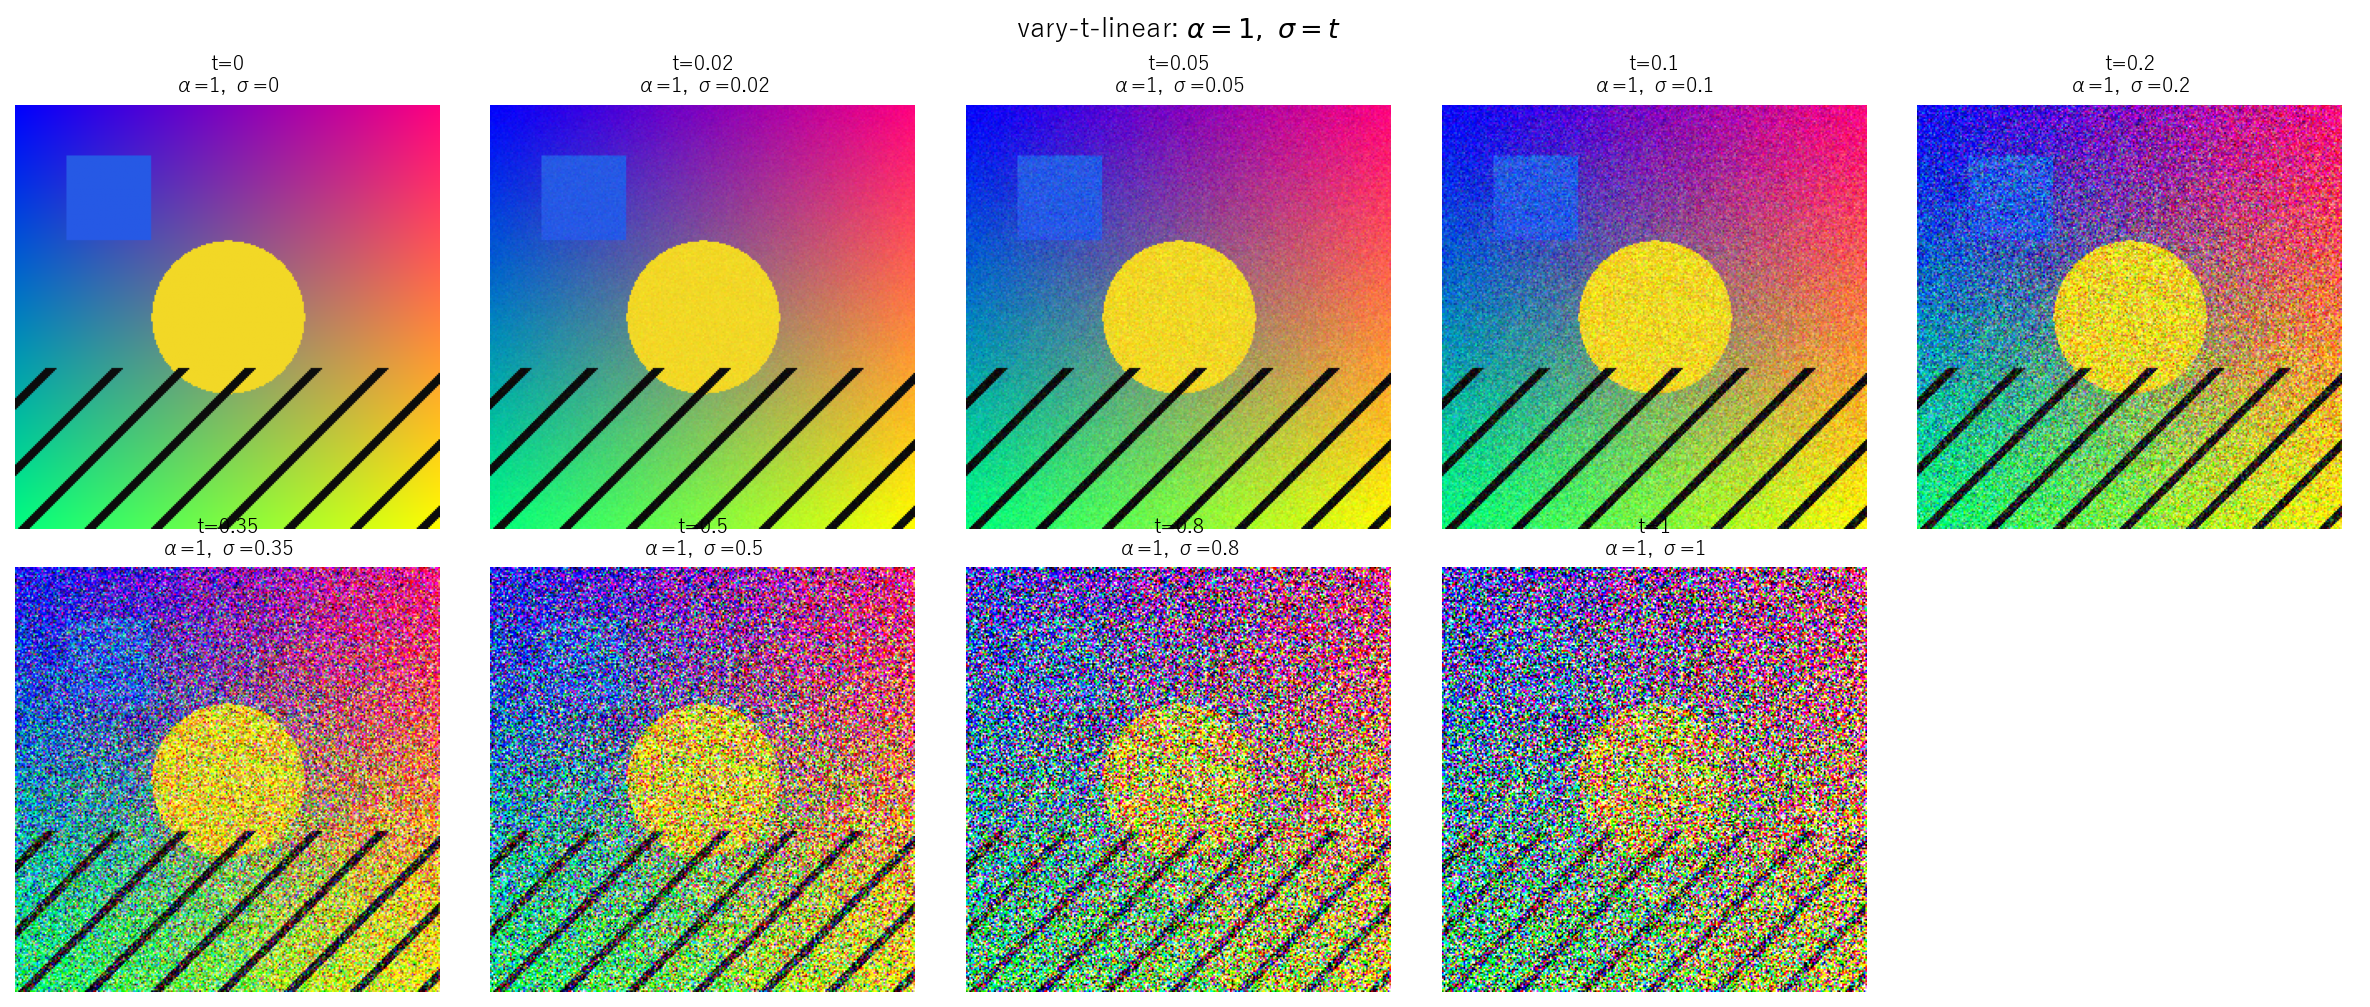
\includegraphics[
        width=\textwidth,
        height=0.72\textheight,
        keepaspectratio
    ]{../experiments/noise-level/vary-t-linear/outputs/grid.png}
    \vspace{0.3em}
    \small 同じ\(\epsilon\)で\(t\)だけを動かす。\(t\approx 0.1\)で粒が見え、\(t=0.5\)以降は形が崩れる。
\end{frame}
%========================================
\begin{frame}{実験：分散一定 \(\alpha^{2}+\sigma^{2}=1\)}
    \centering
    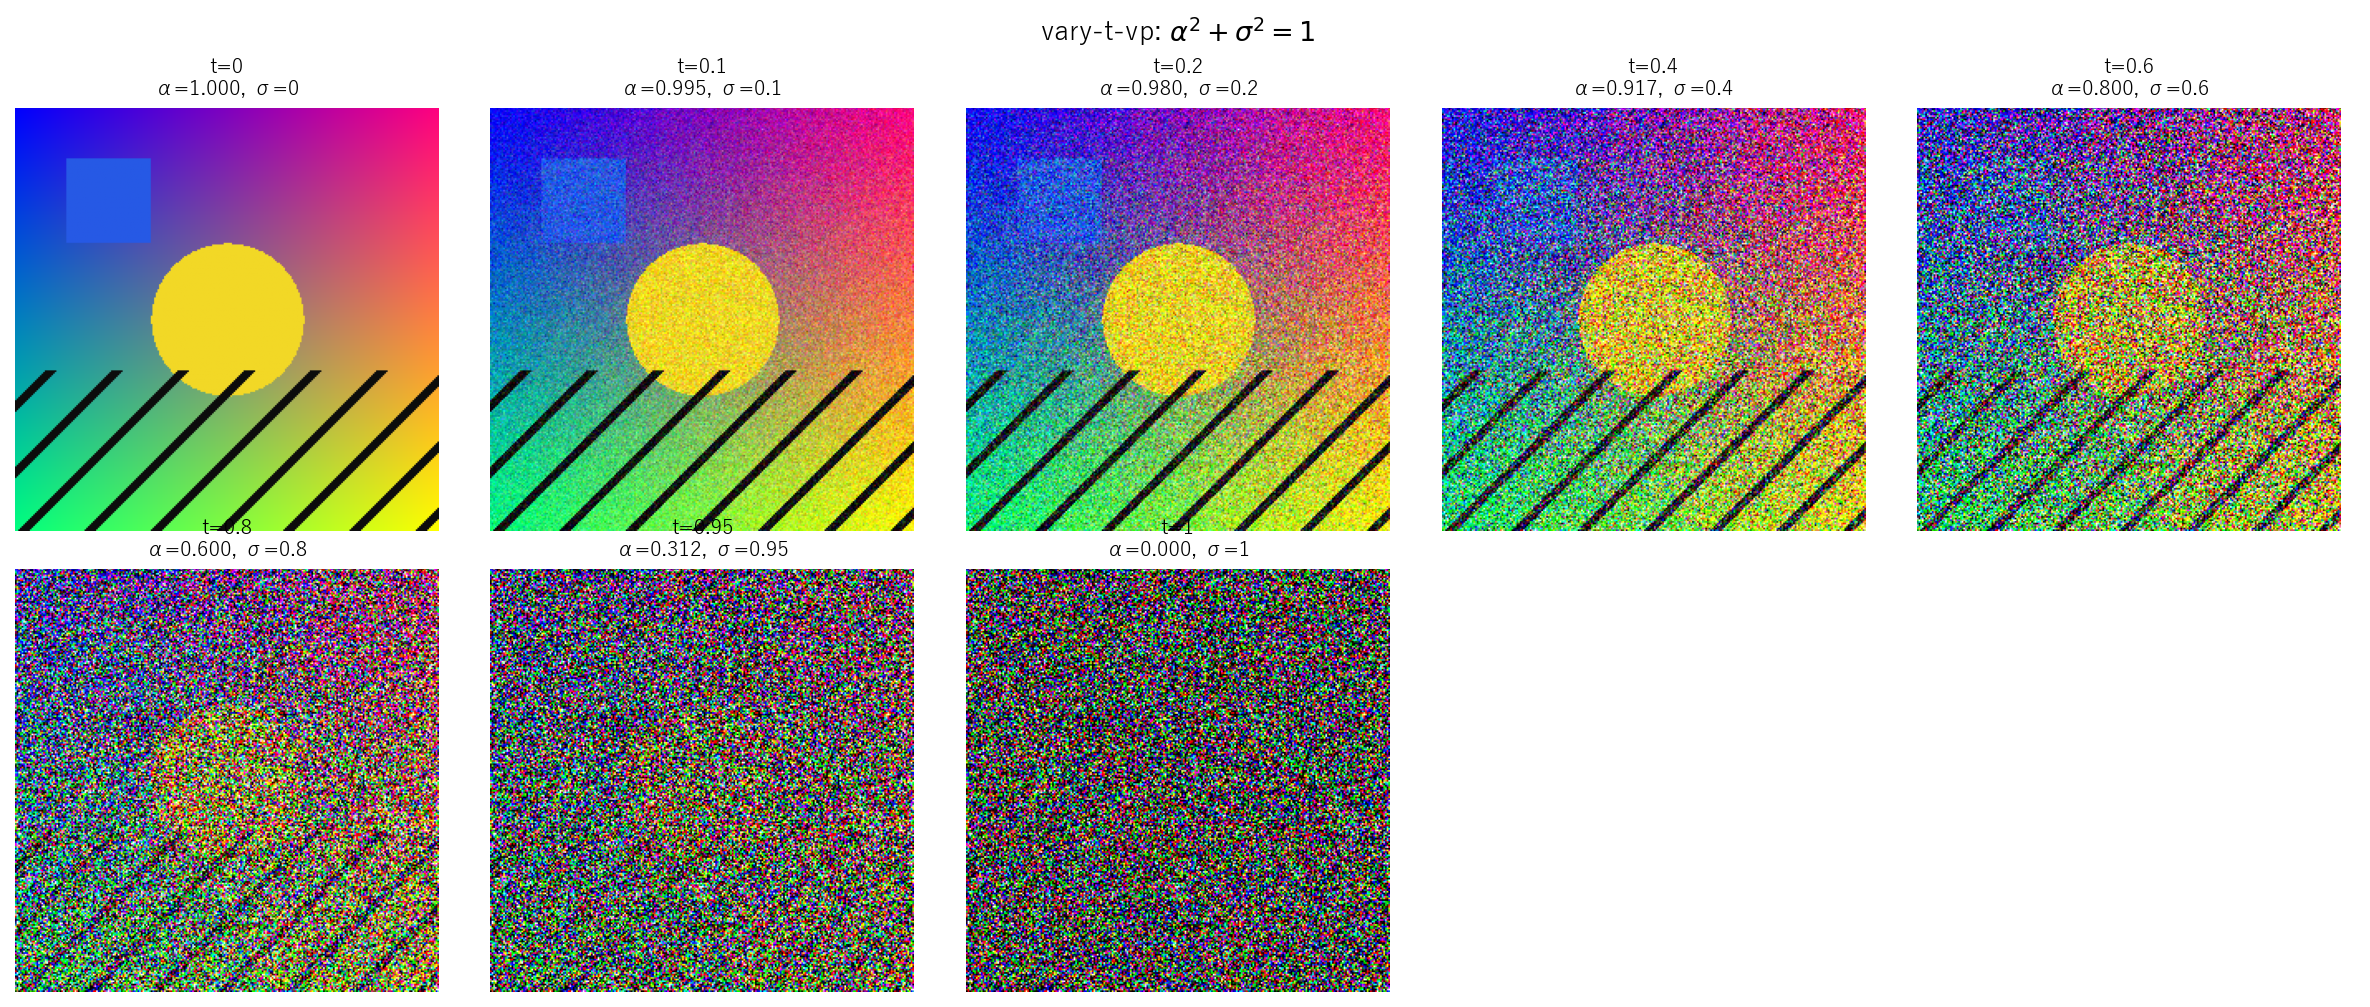
\includegraphics[
        width=\textwidth,
        height=0.72\textheight,
        keepaspectratio
    ]{../experiments/noise-level/vary-t-vp/outputs/grid.png}
    \vspace{0.3em}
    \small \(\sigma=t\)を上げると\(\alpha=\sqrt{1-t^{2}}\)は下がる。\(t=1\)では信号が消え、純ノイズになる。
\end{frame}
%========================================
\begin{frame}{実験：制限なしで\(t>1\)}
    \centering
    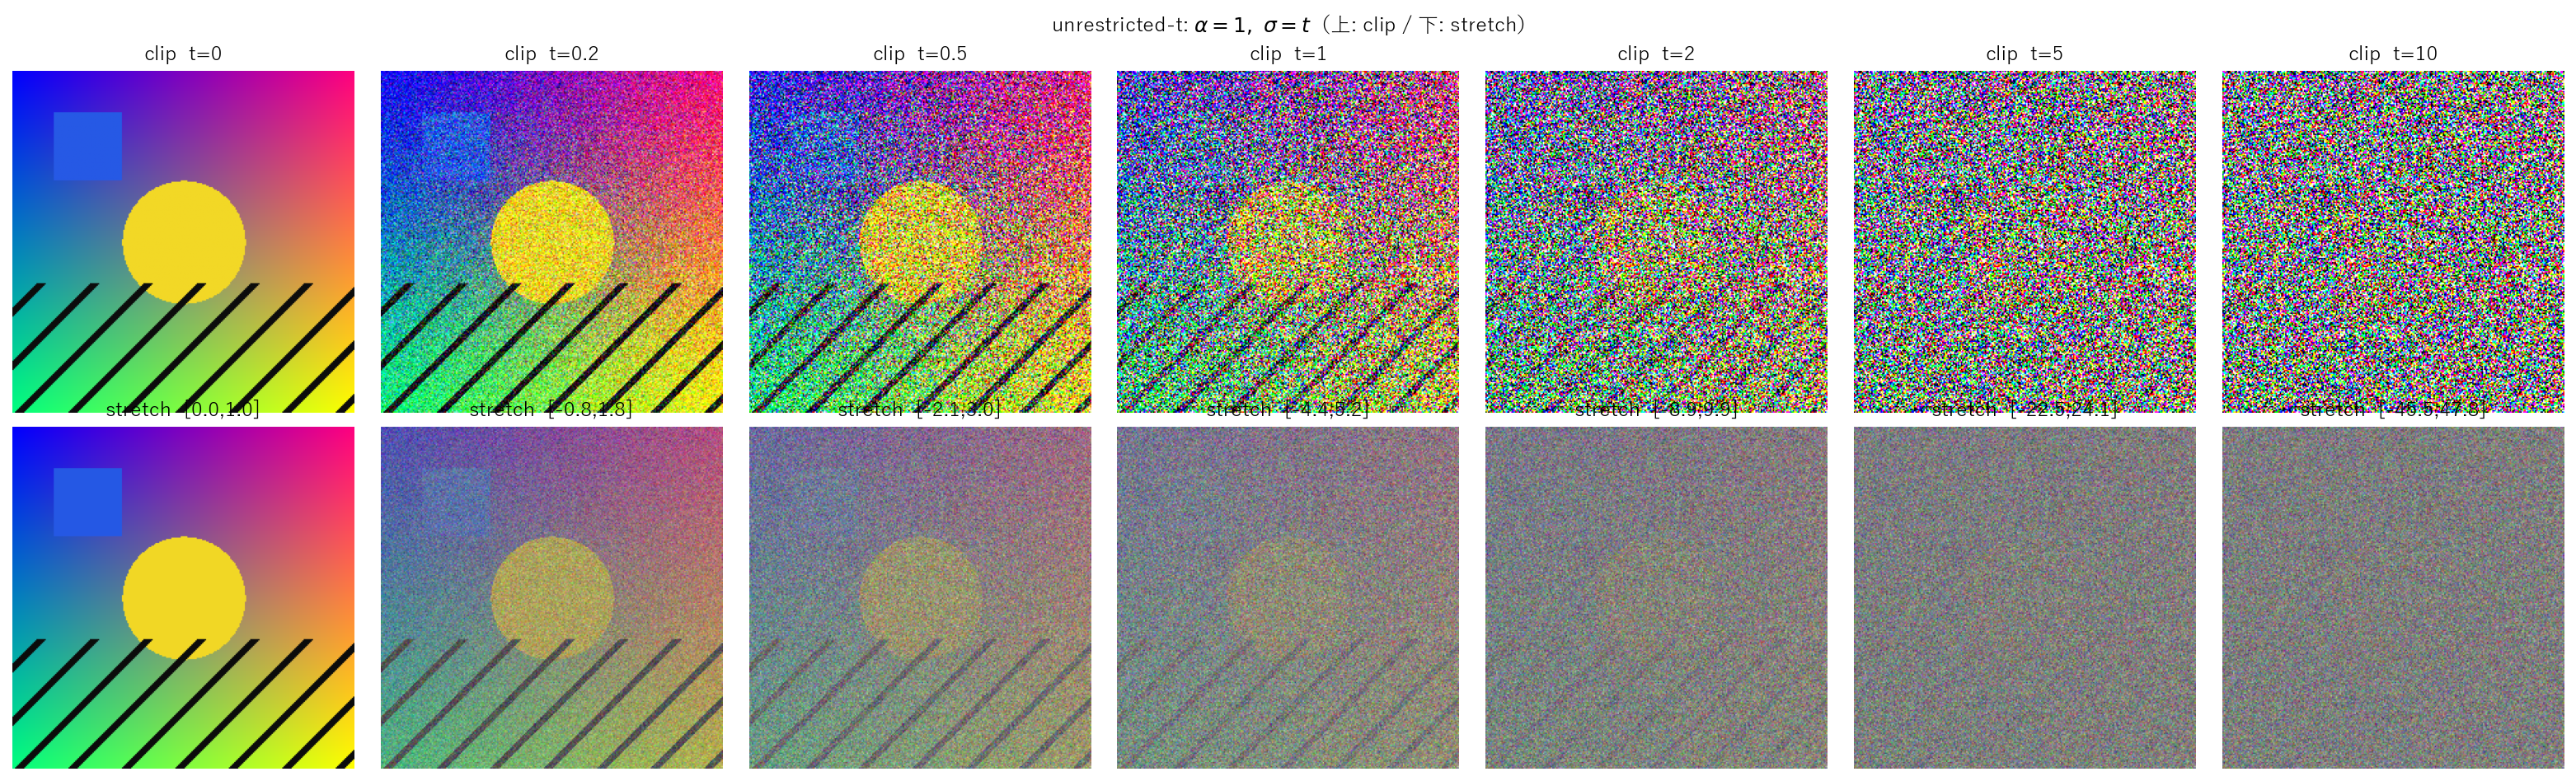
\includegraphics[
        width=\textwidth,
        height=0.78\textheight,
        keepaspectratio
    ]{../experiments/noise-level/unrestricted-t/outputs/grid.png}
    \vspace{0.2em}
    \small 上段は\([0,1]\)へのクリップ、下段は実際の最小〜最大を引き伸ばしたもの。\(t=5,10\)では値が数十まで飛ぶ。
\end{frame}
%========================================
\begin{frame}{実験：\(\sigma\)固定で\(\alpha\)だけ変える}
    \centering
    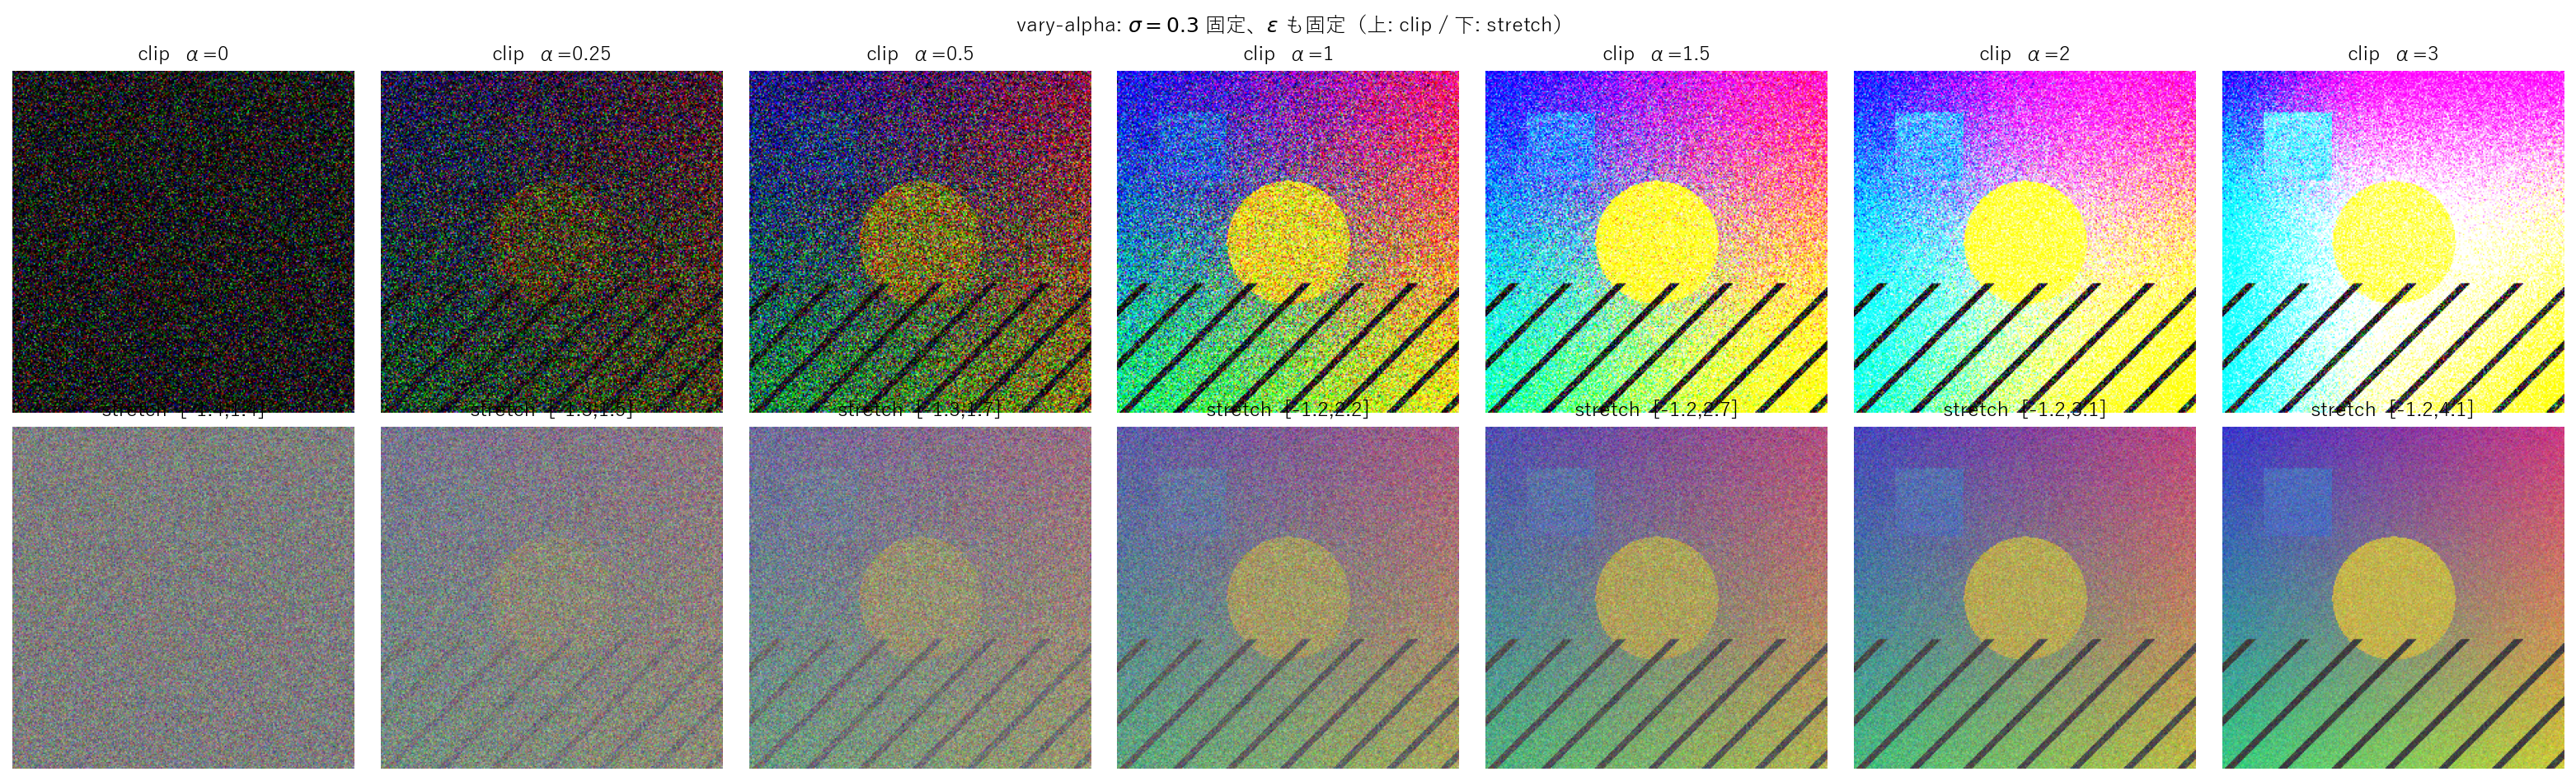
\includegraphics[
        width=\textwidth,
        height=0.78\textheight,
        keepaspectratio
    ]{../experiments/noise-level/vary-alpha/outputs/grid.png}
    \vspace{0.2em}
    \small \(\sigma=0.3\)と\(\epsilon\)は固定。\(\alpha=0\)は純ノイズ、\(\alpha\)を上げると同じ粒の上に元画像が濃く残る。
\end{frame}
%========================================
\begin{frame}{一度の計算と段階的なノイズ付加}
    式\(\boldsymbol{x}_{t}=\alpha_{t}\boldsymbol{x}_{0}+\sigma_{t}\epsilon\)は、選んだノイズレベル\(t\)までに蓄積されたノイズの影響を、一度の計算で直接与える。
    \vspace{0.5em}
    DDPMやスコアに基づく確率微分方程式では、小さなノイズを多数の段階に分けて順番に加えても、そのレベルにおける同じ周辺分布を得られる。
    \vspace{0.5em}
    \begin{exampleblock}{離散的なDDPMの記法}
        後に導入する累積的なノイズ付加は、次のように表す。
        \[
            \boldsymbol{x}_{i}=\bar{\alpha}_{i}\boldsymbol{x}_{0}+\sqrt{1-\bar{\alpha}_{i}^{\,2}}\,\epsilon
        \]
        詳しくは第2.2節と第4章を参照。
    \end{exampleblock}
\end{frame}
%========================================
\begin{frame}{学習：ノイズのない信号を予測する}
    \begin{block}{学習の鍵}
        自分たちでデータにノイズを加えるため、正解を常に把握できる。
    \end{block}
    一つの学習例は、次の手順で作る。
    \begin{itemize}
        \item ノイズのないデータ\(\boldsymbol{x}_{0}\)をサンプリングする
        \item ノイズレベル\(t\)を選ぶ
        \item ノイズ\(\epsilon\)をサンプリングする
    \end{itemize}
    \[
        \boldsymbol{x}_{t}=\alpha_{t}\boldsymbol{x}_{0}+\sigma_{t}\epsilon
    \]
    \(\boldsymbol{x}_{t}\)は自分たちで作ったものなので、どの\(\boldsymbol{x}_{0}\)から生成したのかを正確に把握している。
\end{frame}
%========================================
\begin{frame}{ネットワークに与えるもの}
    ネットワークには\(\boldsymbol{x}_{0}\)も\(\epsilon\)も直接与えない。\\
    与えるのは、ノイズを含む観測データとノイズレベルの組\((\boldsymbol{x}_{t},t)\)だけである。
    \[
        \boldsymbol{x}_{0}^{\mathrm{pred}}:=\boldsymbol{x}_{\phi}(\boldsymbol{x}_{t},t)
    \]
    正解がわかっているため、通常の二乗誤差でこの予測を評価し、改善できる。
    \[
        \bigl\|\boldsymbol{x}_{0}^{\mathrm{pred}}-\boldsymbol{x}_{0}\bigr\|_{2}^{2}
    \]
    \begin{exampleblock}{要点}
        正解となるノイズのないデータと、それにノイズを加えた観測データを用意する。\\
        正解はネットワークに入力せず、観測データから正解を予測できるように学習させる。
    \end{exampleblock}
\end{frame}
%========================================
\begin{frame}{あらゆるノイズレベルでの予測}
    異なるデータサンプル、異なるノイズ、異なるノイズレベルについて、この手順を何度も繰り返す。
    \vspace{0.8em}
    \begin{block}{}
        一つのネットワークが、ほとんどノイズを加えていない状態から、ほぼ純粋なノイズの状態まで、あらゆるノイズレベルで元のデータを予測するように学習する。
    \end{block}
\end{frame}
%========================================
\begin{frame}{二乗誤差のもとで最適な予測}
    二乗誤差のもとで最適な予測は、次のようになる。
    \[
        \boldsymbol{x}_{0}^{*}(\boldsymbol{x}_{t},t)=\mathbb{E}[\boldsymbol{x}_{0}\mid\boldsymbol{x}_{t},t]
    \]
    \small ※ノイズレベルが文脈から明らかな場合、\(\mathbb{E}[\boldsymbol{x}_{0}\mid\boldsymbol{x}_{t}]\)と略記することもある。
    \vspace{0.5em}
    一つのノイズ付き観測データに対応する元のデータは、一意には定まらない。\\
    異なる複数の\(\boldsymbol{x}_{0}\)から、よく似た\(\boldsymbol{x}_{t}\)が生成される可能性がある。
    \vspace{0.4em}
    この曖昧さは\(t>0\)で存在し、ノイズレベルが高くなるとさらに強くなる。\\
    したがってネットワークは、あり得る候補を、その条件付き確率に応じて平均するように学習する。
\end{frame}
%========================================
\begin{frame}{サンプリング：新たなノイズから出発する}
    学習後はパラメータを固定し、それを\(\phi^{\times}\)と呼ぶ。\\
    生成は、これまで説明してきた過程と逆方向に進む。
    \[
        \tilde{\boldsymbol{x}}_{T}\sim p_{\mathrm{prior}}
    \]
    生成途中の状態にはチルダを付けて\(\tilde{\boldsymbol{x}}_{t}\)と表し、\\
    順方向のノイズ付加によって作られる学習用の変数\(\boldsymbol{x}_{t}\)と区別する。
    \vspace{0.6em}
    \begin{alertblock}{この区別が重要である}
        \(\tilde{\boldsymbol{x}}_{T}\)は、隠された実データにノイズを加えて作ったものではない。\\
        その背後には、復元すべき正解の\(\boldsymbol{x}_{0}\)は存在しない。\\
        生成は、特定のデータにノイズを加えた過程を、そのまま逆にたどる操作ではない。
    \end{alertblock}
\end{frame}
%========================================
\begin{frame}{一回のサンプリングステップ}
    現在の状態\(\tilde{\boldsymbol{x}}_{t}\)をネットワークに入力すると、ノイズのないデータの予測が得られる。
    \[
        \boldsymbol{x}_{0}^{\mathrm{pred}}:=\boldsymbol{x}_{\phi^{\times}}(\tilde{\boldsymbol{x}}_{t},t)
    \]
    \(t>0\)では、予測した信号成分を取り除いた残りとして、ノイズ残差も計算できる。
    \[
        \epsilon_{t}^{\mathrm{pred}}:=\frac{\tilde{\boldsymbol{x}}_{t}-\alpha_{t}\boldsymbol{x}_{0}^{\mathrm{pred}}}{\sigma_{t}}
    \]
    この二つは独立した予測ではない。定義上、組み合わせると現在の状態を正確に再構成する。
    \[
        \tilde{\boldsymbol{x}}_{t}=\alpha_{t}\boldsymbol{x}_{0}^{\mathrm{pred}}+\sigma_{t}\epsilon_{t}^{\mathrm{pred}}
    \]
\end{frame}
%========================================
\begin{frame}{ノイズレベルを一段階下げる}
    予測した信号とノイズはそのまま保ち、混ぜる係数だけを少し低いノイズレベル\(t-\Delta t\)のものに変える。
    \[
        \tilde{\boldsymbol{x}}_{t-\Delta t}=\alpha_{t-\Delta t}\boldsymbol{x}_{0}^{\mathrm{pred}}+\sigma_{t-\Delta t}\epsilon_{t}^{\mathrm{pred}}
    \]
    現在の状態に小さな変化を加える式としても書ける。
    \[
        \tilde{\boldsymbol{x}}_{t-\Delta t}
        =\tilde{\boldsymbol{x}}_{t}
        +(\alpha_{t-\Delta t}-\alpha_{t})\boldsymbol{x}_{0}^{\mathrm{pred}}
        +(\sigma_{t-\Delta t}-\sigma_{t})\epsilon_{t}^{\mathrm{pred}}
        \tag{1.4.1}
    \]
    新しい状態\(\tilde{\boldsymbol{x}}_{t-\Delta t}\)を再びネットワークへ入力し、更新された予測を得る。\\
    この処理を\(t=T\)から\(t=0\)まで繰り返すことがサンプリングである。
\end{frame}
%========================================
\begin{frame}{簡単な例：\(\alpha_{t}=1\)、\(\sigma_{t}=t\)}
    先ほどの係数を更新式に代入すると、次のようになる。
    \[
        \tilde{\boldsymbol{x}}_{t-\Delta t}
        =\boldsymbol{x}_{0}^{\mathrm{pred}}
        +(t-\Delta t)\frac{\tilde{\boldsymbol{x}}_{t}-\boldsymbol{x}_{0}^{\mathrm{pred}}}{t}
    \]
    整理すると、単純な加重平均の形になる。
    \[
        \tilde{\boldsymbol{x}}_{t-\Delta t}
        =\frac{t-\Delta t}{t}\tilde{\boldsymbol{x}}_{t}
        +\frac{\Delta t}{t}\boldsymbol{x}_{0}^{\mathrm{pred}}
    \]
    \(\Delta t\)が小さいとき、次の状態は、現在の状態と、ネットワークが予測する最終的なノイズのないデータを混ぜ合わせたものになる。
\end{frame}
%========================================
\begin{frame}{各ステップでの更新}
    各ステップでは、その時点でネットワークが予測するノイズのないデータに向かって、サンプルを少しずつ更新する。
    \vspace{0.8em}
    \begin{alertblock}{「その時点で」が重要である}
        状態を更新すると、ネットワークには新しい、ノイズが少なくなった状態が入力される。\\
        そのため、通常はその予測も変化する。
    \end{alertblock}
    \vspace{0.5em}
    最終的なサンプルは、一回の予測の出力ではない。\\
    直前の更新結果を踏まえて修正される、一連の予測によって作られる。
\end{frame}
%========================================
\begin{frame}{図1.4：拡散モデルによる生成}
    \begin{block}{生成の流れ}
        新たなノイズ\(\tilde{\boldsymbol{x}}_{T}\sim p_{\mathrm{prior}}\)から出発し、\\
        ノイズレベルを下げながらモデルによる予測を繰り返すことで、新しいサンプルを構成する。
    \end{block}
    \vspace{0.6em}
    \begin{exampleblock}{要点}
        新たなノイズから出発し、ノイズのない信号を予測し、\\
        ノイズレベルを下げ、再び予測する。
    \end{exampleblock}
    \vspace{0.6em}
    ※図1.4の画像があれば、\texttt{images}に入れてこのスライドへ埋め込む。
\end{frame}
%========================================
\begin{frame}{最初の予測で終わらない理由}
    最初の予測\(\boldsymbol{x}_{0}^{\mathrm{pred}}\)をそのまま出力して終わりにしてはいけないのか。
    \vspace{0.6em}
    \begin{itemize}
        \item ノイズレベルが高いと、現在の状態にはノイズのないデータの構造に関する情報がほとんど含まれない。\\
        予測は、多数のあり得るサンプルについての大まかな平均に近い
        \item 少し低いノイズレベルへ進むと、曖昧さが少し減った状態をもとに予測できる。\\
        次の予測をより明確にできる
    \end{itemize}
    \vspace{0.5em}
    この処理を何度も繰り返すことで、細部を備えたサンプルが徐々に形成される。
\end{frame}
%========================================
\begin{frame}{以降の章とのつながり}
    \begin{block}{最初の見方}
        ノイズのないデータを予測するという枠組みは、\\
        動作を理解するための最初の見方にすぎない。\\
        ただし、基本的な流れは本書全体を通して共通している。
    \end{block}
    \vspace{0.6em}
    \begin{itemize}
        \item 学習時\\
        ノイズのないデータからノイズ付き観測データを作り、\\
        そこから有用な情報を予測する方法を学ぶ
        \item 生成時\\
        新たなノイズから出発し、ノイズレベルを下げながら、\\
        学習した予測を使って新しいサンプルを構成する
    \end{itemize}
\end{frame}
%========================================
\begin{frame}{以降の章での見方}
    この同じ過程を、異なる数学的な観点から説明する。
    \vspace{0.4em}
    \begin{itemize}
        \item 第2章\\
        DDPMを潜在変数モデルと結び付ける。固定されたノイズ付加過程がエンコーダ、学習された逆方向の遷移がデコーダの役割を果たす
        \item 第3章\\
        ノイズ付きサンプルを更新する方向を与えるスコアを通じて、ノイズ除去を説明する
        \item 第4章\\
        離散的なノイズレベルから連続時間へ移り、逆時間の確率的なダイナミクスによって生成を記述する
        \item 第5章\\
        単純な事前分布からデータ分布への連続的な経路に沿って、サンプルを移動させる過程として生成を捉える
        \item 第6章\\
        これらの見方がどのようにつながっているのかを説明する
    \end{itemize}
\end{frame}